\documentclass[10pt]{scrreprt}
\usepackage[utf8]{inputenc}
\usepackage{amsfonts}
\usepackage{amsmath}
\usepackage{amssymb}
\usepackage{commath}
\usepackage[ngerman]{babel}
\usepackage{enumitem}
\usepackage{booktabs}
\usepackage{longtable}
\usepackage{relsize}
\usepackage{pgfplots}
\usepackage{csvsimple}
\usepackage{pgfplotstable}
\usepackage{siunitx}
\usepackage{fancyhdr}
\usepackage{color}
\usepackage{float}
\usepackage{listings}

\definecolor{mygreen}{RGB}{28,172,0} % color values Red, Green, Blue
\definecolor{mylilas}{RGB}{170,55,241}


\lstset{language=Matlab,%
    %basicstyle=\color{red},
    breaklines=true,%
    morekeywords={matlab2tikz},
    keywordstyle=\color{blue},%
    morekeywords=[2]{1}, keywordstyle=[2]{\color{black}},
    identifierstyle=\color{black},%
    stringstyle=\color{mylilas},
    commentstyle=\color{mygreen},%
    showstringspaces=false,%without this there will be a symbol in the places where there is a space
    %numbers=left,%
    %numberstyle={\tiny \color{black}},% size of the numbers
    %numbersep=9pt, % this defines how far the numbers are from the text
    emph=[1]{for,end,break},emphstyle=[1]\color{red}, %some words to emphasise
    %emph=[2]{word1,word2}, emphstyle=[2]{style},
}

\setlength\parindent{0pt}

\setcounter{chapter}{3}
\setcounter{secnumdepth}{3}
\setcounter{figure}{12}


\pagestyle{fancy}
\fancyhf{}
\lhead{GPET Versuch 4}
\rhead{Tim Luchterhand, Paul Nykiel}
\cfoot{\thepage}

\author{Tim Luchterhand, Paul Nykiel \protect\\ tim.luchterhand@uni-ulm.de, paul.nykiel@uni-ulm.de}
\title{GPET Versuch 4 --- Henry meets Faraday}
\subtitle{Gruppe: Dienstag14}

\begin{document}
        \maketitle
        \section{Ein- und Ausschaltvorgang einer Induktivität}
        \paragraph{Einführung}
        In diesem Versuch sollen die zeitlichen Verläufe des Stromes und der Spannung beim
        Schalten einer Induktivität untersucht werden. Verwenden Sie hierzu den in Abbildung
        ~\ref{fig:abb13} gezeigten Versuchsaufbau. Verwenden Sie einen Widerstand von $R=100\si{\ohm}$ und die
        Spule mit $n=250$ Windungen. Stellen Sie eine Rechteckspannung mit $f=10\si{k\hertz}$ ein.
        Bestimmen Sie den Verlauf der Spannung an der Spule, $U_2$, sowie des Stromes durch die
        Spule (über die Differenz der Spannungen $U_1$ und $U_2$) mit Hilfe des Oszilloskops und
        erklären Sie den charakteristischen Verlauf beider Größen.
        \begin{center}
            \begin{figure}[H]
                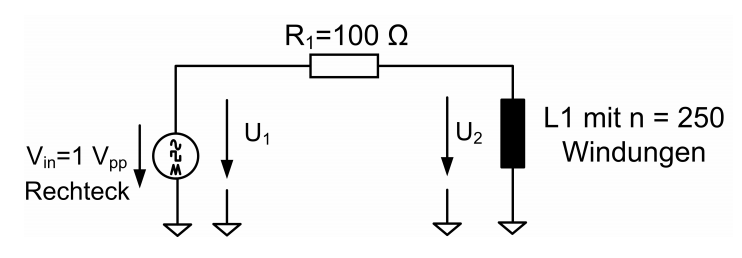
\includegraphics[width=\textwidth]{Abbildung13.png}
                \caption{Messaufbau um Strom- und Spannungsverlauf beim Schalten der Spannung
an einer Spule zu bestimmen}
                \label{fig:abb13}
            \end{figure}
        \end{center}

        \subsection{Versuchsauswertung}

        \subsubsection{Screenshot}
        \paragraph{Aufgabe}
        Erstellen Sie einen Screenshot der Spannungs- und Stromverläufe.

        \paragraph{Protokoll}
        $U_1$ in \textcolor{green}{grün}, $U_2$ in \textcolor{yellow}{gelb}
        $U_1 - U_2 = I \cdot R_1$ in \textcolor{violet}{violett}.
        \begin{center}
            \begin{figure}[H]
                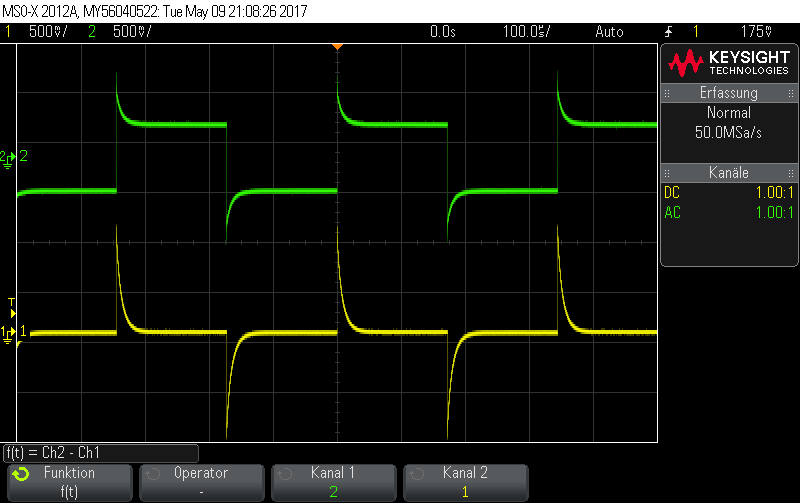
\includegraphics[width=\textwidth]{scope_2.png}
                \caption{Spannung an der Spule}
                \label{fig:spannspul}
            \end{figure}
        \end{center}

        Die Eingangsspannung $U_1$ steigt zu beginn eines Duty-cyles auf den
        eingestellten Maximalwert an, fällt dann aber exponentiell auf einen tieferen
        Wert ab und verläuft schließlich konstant. Dies lässt sich wie folgt erklären:
        Bei der ansteigenden Flanke der Rechteckspannung verhält sich die Induktivität
        wie ein Leerlauf. Die Spannung steigt also auf das eingestellte Maximum. Der Strom,
        der durch die Induktivität fließt, steigt im weiteren Verlauf wie folgt an:
        \begin{equation}
            I_L(t) = \frac{U_{eingang}}{R}\left(\exp{\left(-\frac{Rt}{L}\right)} - 1\right)
            \label{eq:ISpule}
        \end{equation}

        Dadurch fällt $U_1$ exponentiell ab. Der konstante Verlauf von $U_1$ stellt sich
        dann ein, wenn der Sättigungsstrom der Spule erreicht ist. Die gemessene Spannung
        berträgt dann die Spannung am Widerstand R.

        $U_2$ verhält sich identisch zu $U_1$. Der einzige Unterschied ist, dass die Spannung
        auf $0\si{\volt}$ abfällt, da über der gesättigten Spule keine Spannung mehr abfällt.

        Der Ausschaltvorgang verhält sich analog.
        \begin{center}
            \begin{figure}[H]
                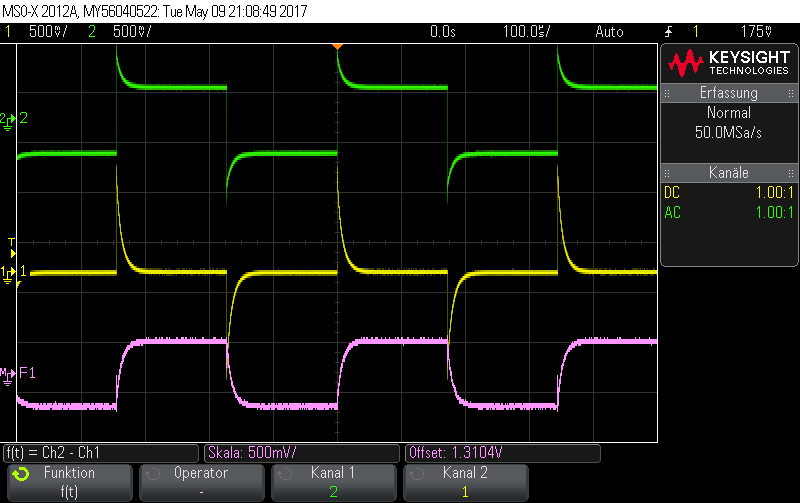
\includegraphics[width=\textwidth]{scope_3.png}
                \caption{Strom (in violett) an der Spule}
            \end{figure}
        \end{center}

        Der Strom, der durch die Spule fließt, lässt sich wie folgt bestimmen:
        \begin{equation}
            I_L = \frac{U_1 - U_2}{R}
        \end{equation}

        Im Diagramm ist lediglich die Spannungsdifferenz in violett dargestellt. Diese
        ist jedoch proportional zum Kehrwert des Widerstandes R. Der Strom verhält sich
        wie durch Gleichung~\ref{eq:ISpule} beschrieben und steigt exponentiell auf einen Sättigungsstrom
        an.

        Der Ausschaltvorgan verhält sich analog.


        \section{Freie Schwingungen}
        \paragraph{Einführung}
        In diesem Versuch werden die freien Schwingungen eines LC Schwingkreises genauer untersucht.

        \subsection{Parasitäre Kapazität}
        \paragraph{Aufgabe}
        Bauen Sie hierzu zunächst die in Abbildung~\ref{fig:abb14} gezeigte Schaltung auf. Verwenden
        Sie die Spule mit $n = 1000$ Windungen.
        \begin{center}
            \begin{figure}[H]
                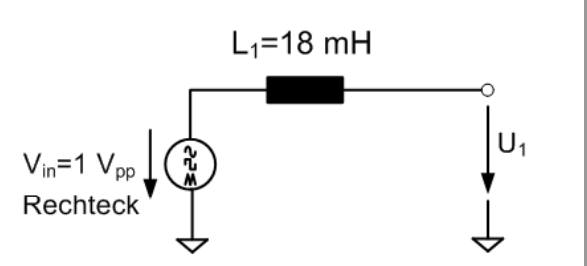
\includegraphics[width=\textwidth]{Abbildung14.png}
                \caption{Messaufbau zur Erzeugung einer freien Schwingung uber die Eigenresonanz einer Spule.}
                \label{fig:abb14}
            \end{figure}
        \end{center}

        \paragraph{Bemerkung}
        Die beobachtete Schwingung kommt durch die sogenannte Eigenresonanz der verwendeten
        Spule zu Stande. Die Spule weist neben ihrer Induktivität und ihrem
        Widerstand auch eine parasitäre Kapazität gemäß Abbildung 15 auf. Diese führt
        dazu, dass die Spule für höhere Frequenzen nicht mehr als reine Induktivität wirkt
        sondern sich wie ein gedämpfter parallel-LC-Schwingkreis verhält.

        \begin{center}
            \begin{figure}[H]
                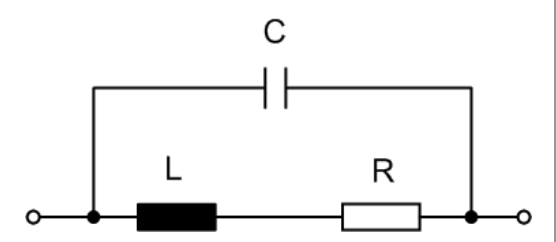
\includegraphics[width=\textwidth]{Abbildung15.png}
                \caption{Ersatzschaltbild einer realen Spule mit parasitärem Widerstand und parasitärer Kapazität.}
                \label{fig:abb15}
            \end{figure}
        \end{center}

        \paragraph{Aufgabe}
        Nehmen Sie den Verlauf der Spannung $U_1$ mit dem Oszilloskop auf und verwenden
        Sie die Cursorfunktion des Oszilloskops, um die Frequenz der Schwingung sowie die
        Abnahme der Amplitude der Schwingung zu messen.

        \subsubsection{Screenshot}
        \paragraph{Aufgabe}
        Erstellen Sie für Ihre Versuchsauswertung einen Screenshot der Messung.

        \paragraph{Protokoll}
        \begin{center}
            \begin{figure}[H]
                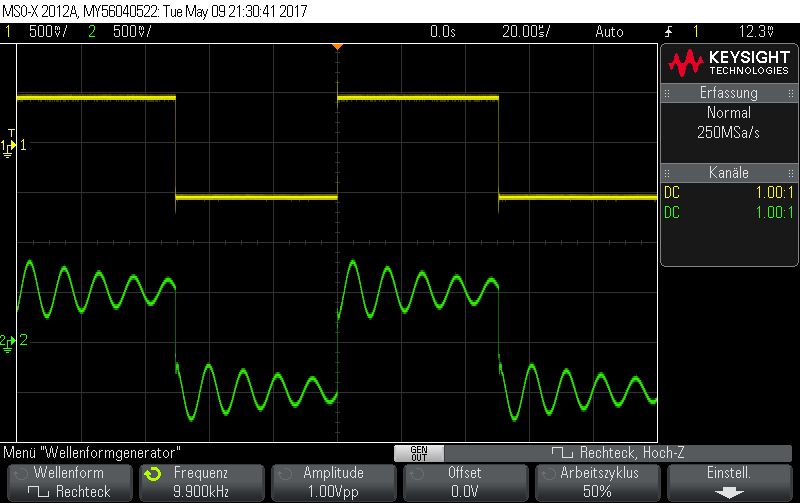
\includegraphics[width=\textwidth]{scope_8.png}
                \caption{Spannung an der Spule}
            \end{figure}
        \end{center}

        Es fällt auf, dass das grüne Spulensignal ($U_1$) sich nicht verhält wie
        ein typischer Einschaltvorgang an einer Spule, sondern eine gedämpfte
        harmonische Schwingung ausführt.

        \textbf{Erklärung:} Die Spule, die neben ihrer Induktivität auch noch eine
        parasitäre Kapazität aufweißt, führt bei Resonanzfrequenz eine harmonische
        Schwingung aus, die durch den ohmschen Widerstand der Spule gedämpft wird.

        \subsubsection{Abschätzung der Kapazität}
        \paragraph{Aufgabe}
        Schätzen Sie mit Hilfe Ihrer Messung den Wert der parasitären Kapazität der
        verwendeten Spule ab.

        \paragraph{Protokoll}
        \begin{center}
            \begin{figure}[H]
                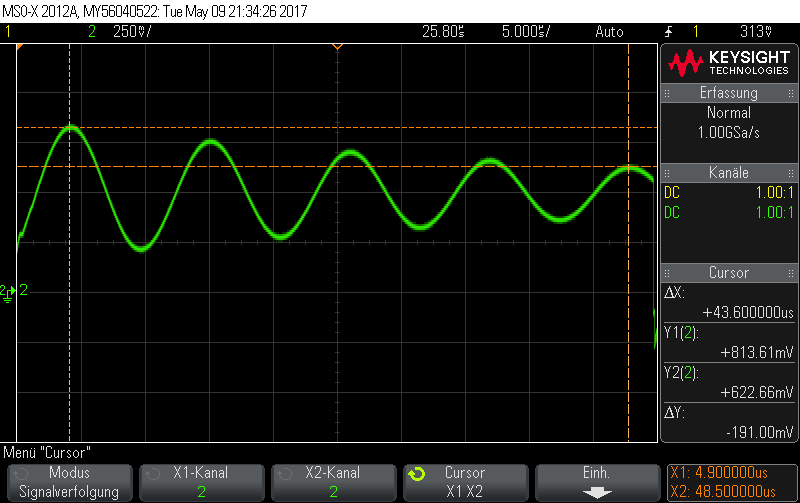
\includegraphics[width=\textwidth]{scope_9.png}
                \caption{Spannung an der Spule}
            \end{figure}
        \end{center}

        \paragraph{Vorgehensweise}
        Mit Cursor wird die Frequenz des LC-Schwingkreises bestimmt. Um eine höhere
        Genauigkeit zu erzielen, wurden 5 Perioden gemessen und der Durchschnitt
        berechnet. Durch folgende Formeln lässt sich dann die parasitäre Kapazität
        abschätzen.

        \begin{eqnarray}
            \Delta x &=& 43.6\si{\mu\second}\\
            f_0 &=& \frac{5}{\Delta x} = 114.678\si{k\hertz}\\
            f_0 &=& \frac{1}{2 \pi \sqrt{L C}}\\
            \Leftrightarrow C &=& \frac{1}{{(2 \pi f_0)}^2 L} \approx 0.11\si{n\farad}
        \end{eqnarray}
        %@TODO rgebnis, kleine Kap usw.

        \subsection{Schwingung am Kondensator}
        Bauen Sie als nächstes die in Abbildung~\ref{fig:abb16} dargestellte Schaltung auf. Verwenden
        Sie erneut die Spule mit $n = 1000$ Windungen und den Kondensator mit $C_1 =
        100 \si{\farad}$.

        \begin{center}
            \begin{figure}[H]
                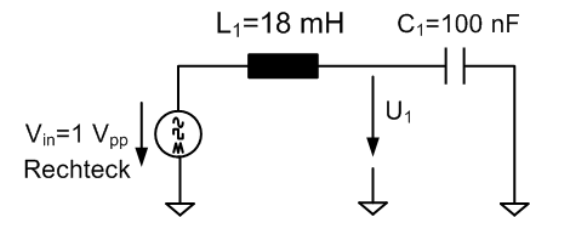
\includegraphics[width=\textwidth]{Abbildung16.png}
                \caption{Messaufbau zur Erzeugung einer freien Schwingung in einem Serien LC-Schwingkreis.}
                \label{fig:abb16}
            \end{figure}
        \end{center}

        \paragraph{Aufgabe}
        Nehmen Sie den Verlauf der Spannung $U_1$ mit dem Oszilloskop auf und verwenden
        Sie die Cursorfunktion des Oszilloskops, um die Frequenz der Schwingung
        sowie die Abnahme der Amplitude der Schwingung zu messen.

        \vspace{0.5cm}

        Erstellen Sie für Ihre Versuchsauswertung einen Screenshot der Messung.

        \paragraph{Protokoll}
        \begin{center}
            \begin{figure}[H]
                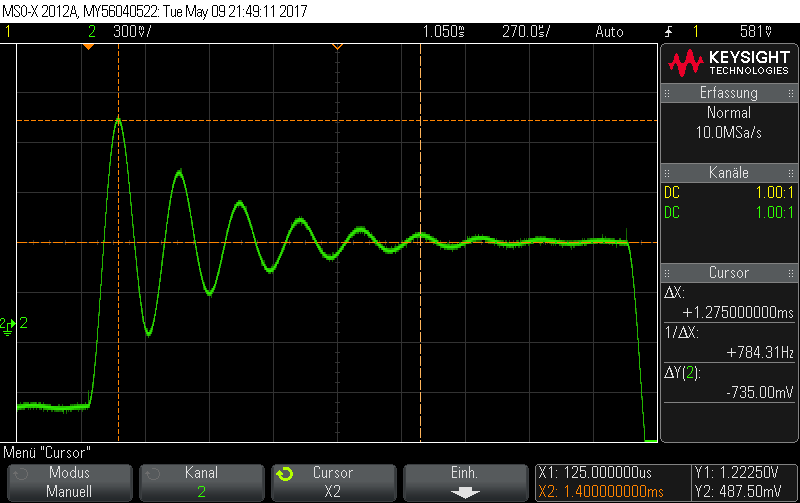
\includegraphics[width=\textwidth]{scope_12.png}
                \caption{Spannung am Kondensator}
            \end{figure}
        \end{center}

        Das Bild zeigt die Spannung am Kondensator des LC-Kreises bei einer
        steigenden Rechteckflanke des Eingangssignals.
        Es ist eine gedämpfte harmonische Schwingung zu erkennen.

        Aus Genauigkeitsgründen wurden fünf Perioden gemessen. Der Messcursor
        wurde auf das jeweilige Maximum gesetzt, da die Nulldurchgänge ohne eine
        klare Nullreferenz schwer zu bestimmen sind.

        Die Frequenz lässt sich dann wie folgt wie berechnen:
        \begin{center}
            \begin{eqnarray}
                \Delta x &=& 1.275 \si{m \second}\\
                f_0 &=& \frac{5}{\Delta x} \approx 3922\si{\hertz}\\
            \end{eqnarray}
            \begin{figure}[H]
                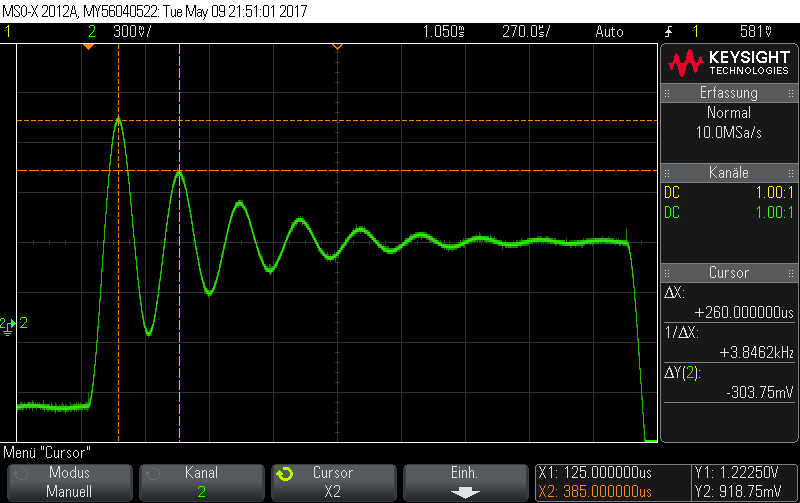
\includegraphics[width=\textwidth]{scope_13.png}
                \caption{Abnahme der Amplitude der Schwingung des LC-Schwingkreises}
                \label{fig:SpanAbn}
            \end{figure}
        \end{center}

        Aus~\ref{fig:SpanAbn} lassen sich die ersten beiden Amplituden der Schwingung
        bestimmen. Folgendermaßen lässt sich dann eine Exponentialfunition aufstellen,
        die den Verlauf der Amplitude beschreibt.

        \begin{eqnarray}
            \hat{U}_1 &=& 735\si{m\volt}\\
            \hat{U}_2 &=& \hat{U_1} - 303.75\si{m\volt} = 431.25\si{m\volt}\\
            \alpha &=& \frac{\hat{U_2}}{\hat{U_1}} = 0.587\\
            \hat{U}(t) &=& \alpha^{\dfrac{t}{\Delta x}} = \exp{(\log{(\alpha)} \cdot \frac{t}{\Delta x})}
        \end{eqnarray}

        \subsection{Veränderung der Schwingung}
        \paragraph{Aufbau}
        Bauen Sie nun die in Abbildung~\ref{fig:abb17} gezeigte Schaltung auf. Verwenden Sie erneut
        die Spule mit $n = 1000$ Windungen und den Kondensator mit $C_1 = 100\si{n\farad}$ sowie
        als Widerstand das Potentiometer.
        \begin{center}
            \begin{figure}[H]
                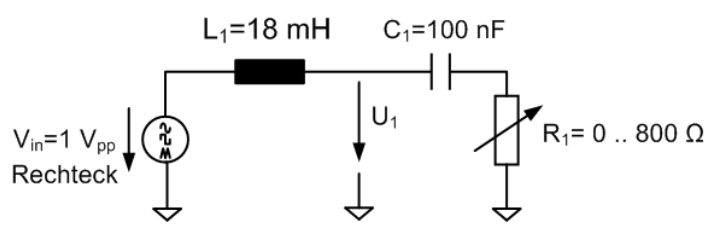
\includegraphics[width=\textwidth]{Abbildung17.png}
                \caption{Messaufbau Erzeugung einer freien Schwingung in einem Serien-LC Schwingkreis
                        mit erhöhter Dämpfung.}
                \label{fig:abb17}
            \end{figure}
        \end{center}

        \subsubsection{Spannungsverlauf}
        \paragraph{Aufgabe}
        Nehmen Sie den Verlauf der Spannung $U_1$ mit dem Oszilloskop auf. Stellen Sie
        mit dem Potentiometer nacheinander verschiedene Widerstandswerte zwischen
        $0$ und $800\si{\ohm}$ ein. Beobachten und beschreiben Sie die Änderungen im Verlauf
        der Schwingung.

        \paragraph{Protokoll}
        \begin{center}
            \begin{figure}[H]
                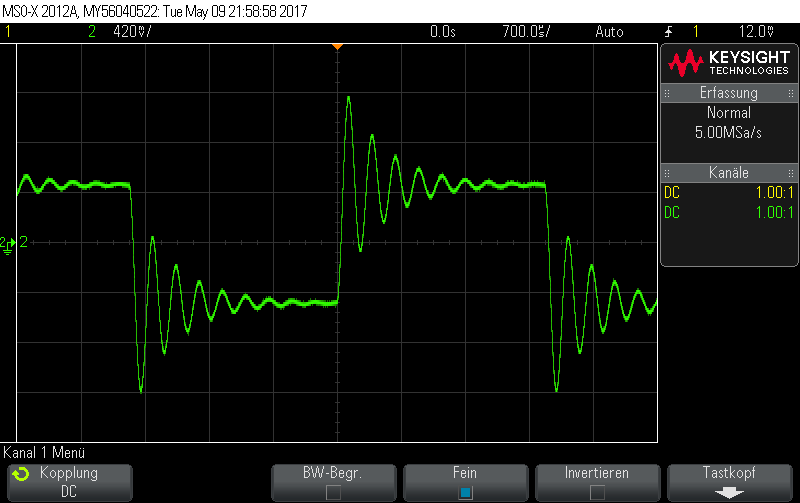
\includegraphics[width=\textwidth]{scope_14.png}
                \caption{Potentiometer mit $R = 0\si{\ohm}$}
            \end{figure}
            \begin{figure}[H]
                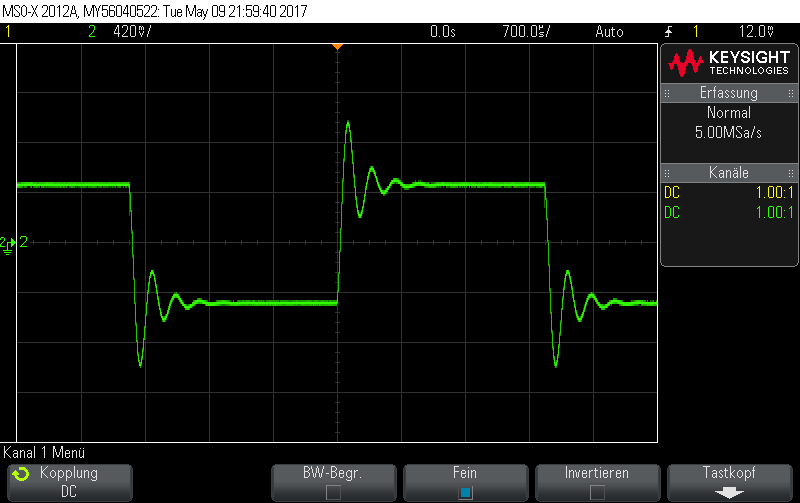
\includegraphics[width=\textwidth]{scope_15.png}
                \caption{Potentiometer mit $R = 100\si{\ohm}$}
            \end{figure}
            \begin{figure}[H]
                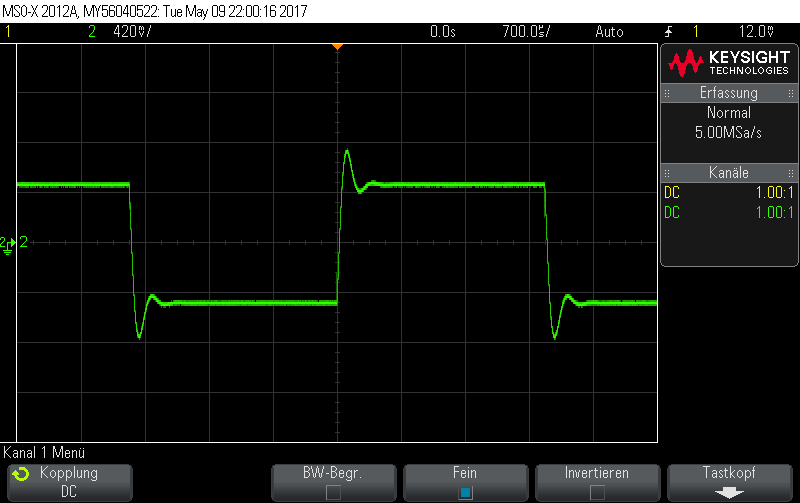
\includegraphics[width=\textwidth]{scope_16.png}
                \caption{Potentiometer mit $R = 300\si{\ohm}$}
            \end{figure}
            \begin{figure}[H]
                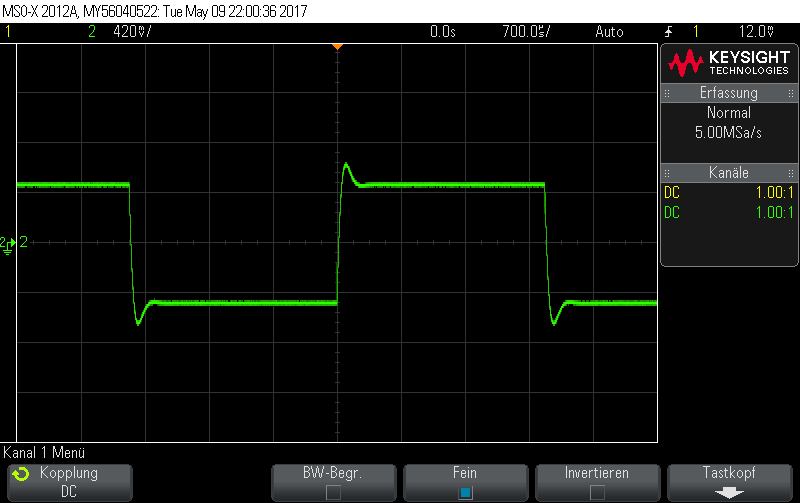
\includegraphics[width=\textwidth]{scope_17.png}
                \caption{Potentiometer mit $R = 500\si{\ohm}$}
            \end{figure}
            \begin{figure}[H]
                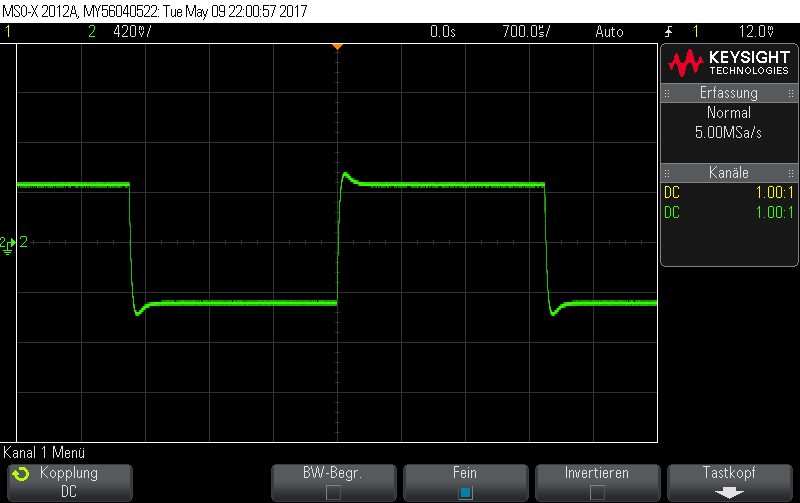
\includegraphics[width=\textwidth]{scope_18.png}
                \caption{Potentiometer mit $R = 800\si{\ohm}$}
            \end{figure}
        \end{center}

        Durch Erhöhen des Widerstandes des Potentiometers wird die Amplitude
        der Schwingung verringert. Der Widerstand fungiert also als Dämpfung
        und verändert nur die Amplitude und hat keinen Einfluss auf die Frequenz
        oder Phase der Schwingung. Bei einem Widerstand von $800 \si{\ohm}$ ist
        die Dämpfung so groß, dass die Schwingung kaum noch zu erkennen ist.


        \subsubsection{Screenshot}
        \paragraph{Aufgabe}
        Nehmen Sie nun für einen Wert von $R_1 \approx 15\si{\ohm}$ den Verlauf der Spannung $U_1$
        mit dem Oszilloskop auf und verwenden Sie die Cursorfunktion des Oszilloskops,
        um die Frequenz der Schwingung sowie die Abnahme der Amplitude
        der Schwingung zu messen. Erstellen Sie für Ihre Versuchsauswertung einen
        Screenshot dieser Messung.

        \paragraph{Protokoll}
        \begin{center}
            \begin{figure}[H]
                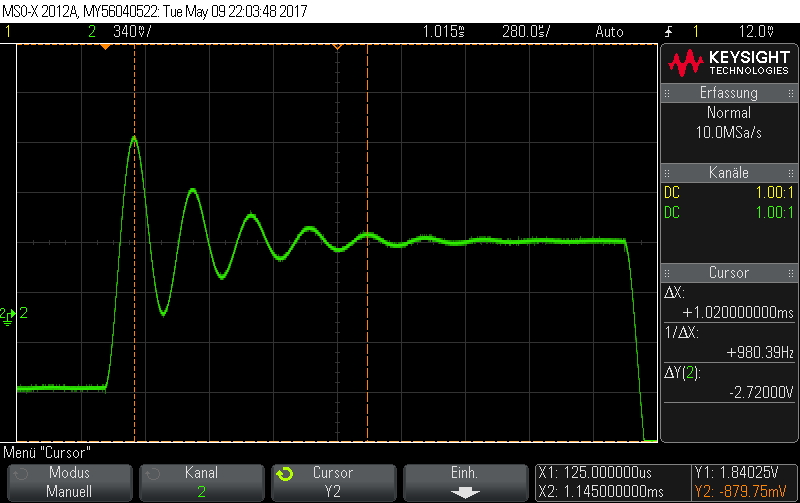
\includegraphics[width=\textwidth]{scope_19.png}
                \caption{Bestimmung der Frequenz}
            \end{figure}
        \end{center}

        Das Bild zeigt die Spannung die über Kondensator und
        Potentiometer des LC-Kreises bei einer
        steigenden Rechteckflanke des Eingangssignals abfällt.
        Es ist eine gedämpfte harmonische Schwingung zu erkennen.

        Aus Genauigkeitsgründen wurden fünf Perioden gemessen. Der Messcursor
        wurde auf das jeweilige Maximum gesetzt, da die Nulldurchgänge ohne eine
        klare Nullreferenz schwer zu bestimmen sind.

        Die Frequenz lässt sich dann wie folgt wie berechnen:
        \begin{eqnarray}
            \Delta x &=& 1.02 \si{m \second}\\
            f_0 &=& \frac{5}{\Delta x} \approx 4902\si{\hertz}\\
        \end{eqnarray}
        \begin{center}
            \begin{figure}[H]
                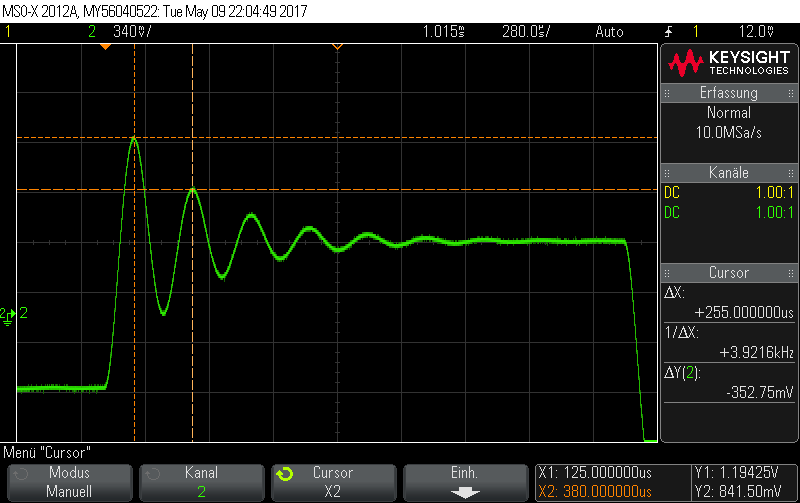
\includegraphics[width=\textwidth]{scope_20.png}
                \caption{Abnahme der Amplitude}
                \label{fig:SpanAbn2}
            \end{figure}
        \end{center}

        In der ersten Periode nimmt die Amplitude um $352.75 \si{m \volt}$ ab.

        \section{Spannungsüberhöhung}
        \paragraph{Aufgabe}
        In folgender Messung soll der Effekt der Spannungsüberhöhung in einem Serien-LC Schwingkreis
        untersucht werden. Errichten Sie hierzu die Schaltung nach Abbildung
        \ref{fig:abb18}. Verwenden Sie die Spule mit $n = 1000$ Windungen sowie einen Kondensator mit
        $C = 100\si{n\farad}$.

        \begin{center}
            \begin{figure}[H]
                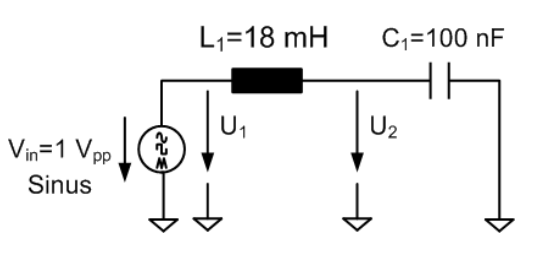
\includegraphics[width=\textwidth]{Abbildung18.png}
                \caption{Messaufbau zur Untersuchung der Spannungsüberhöhung in einem
                    Serien-LC-Schwingkreis.}
                \label{fig:abb18}
            \end{figure}
        \end{center}

        \subsection{Spannungsmaximum}
        \paragraph{Aufgabe}
        Bei welcher Frequenz erwarten Sie ein Maximum der Spannung $U_2$? Begrunden Sie
        Ihre Antwort.

        \paragraph{Protokoll}
        Die maximale Amplitude wird bei der Resonanzfrequenz $f_0$ erreicht. Diese lässt
        sich wie folgt berechnen:
        \begin{eqnarray}
            f_0 &=& \frac{1}{\sqrt{LC}} = 3.751\si{k\hertz}\\
        \end{eqnarray}

        \subsection{Frequenzsweep}
        \paragraph{Aufgabe}
        Führen Sie mit Hilfe der MATLAB GUI einen Sweep der Eingangsfrequenz durch.
        Verwenden Sie dafür folgende Parameter: Type: Sweep frequency, peak-to-peak;
        Frequency sweep: logarithmic; Spannung 2 Vpp; Frequenz: 200 Hz bis 10 kHz; Anzahl
        der Punkte: 50. Fügen Sie eine Messkurve aus der GUI in Ihre Auswertung bei.
        Erzeugen Sie eine Grafik des durchgeführten Sweeps.

        \paragraph{Protokoll}
        \begin{center}
            \begin{figure}[H]
                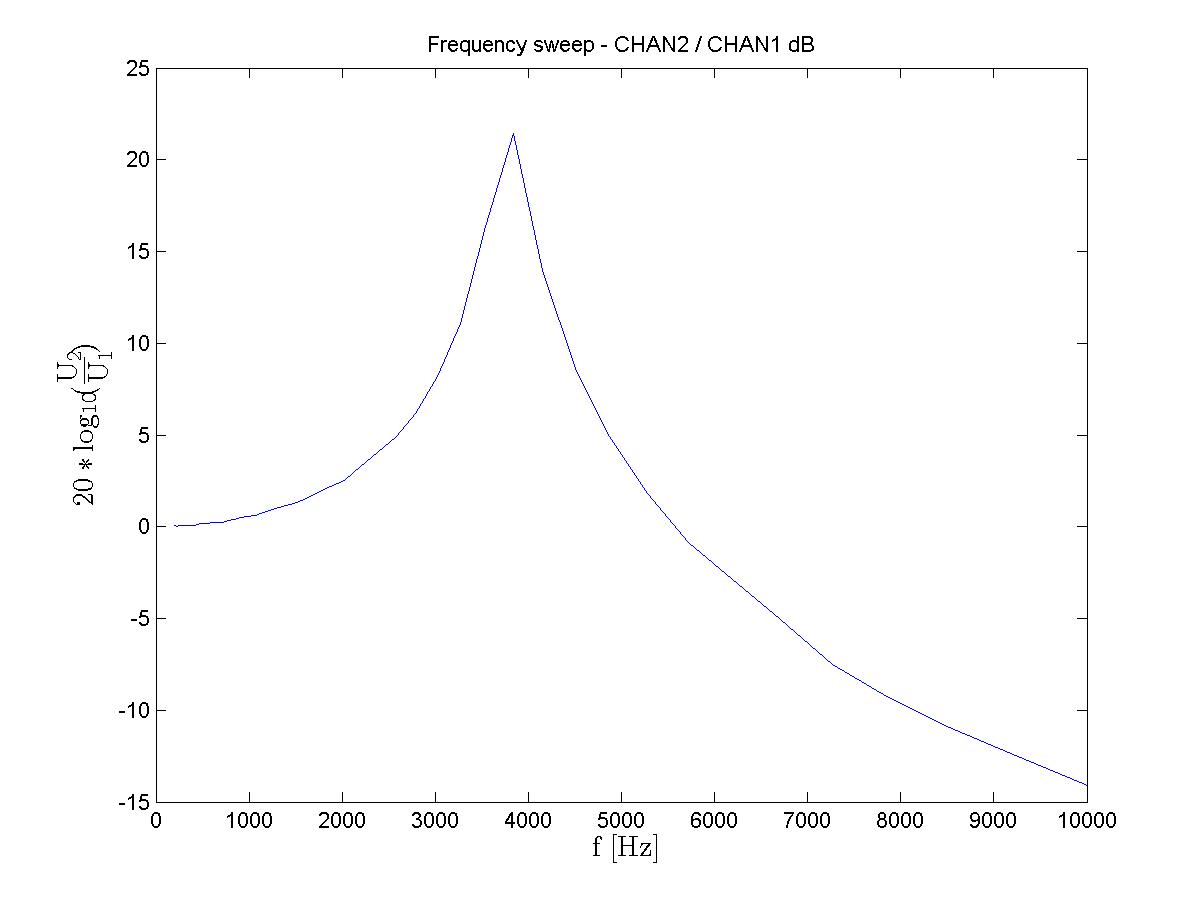
\includegraphics[width=\textwidth]{F_Sweep_1_frequencysweep_ylogxlin.jpg}
                \caption{Frequenzsweep}
                \label{fig:fsweep1}
            \end{figure}
        \end{center}
        \subsection{Übereinstimmung mit den theoretischen Werten}
        \paragraph{Aufgabe}
        Stimmt die Messung mit dem theoretischen Wert überein?

        \paragraph{Protokoll}
        Wie in Diagramm~\ref{fig:fsweep1} zu erkennen, erhält man die größte Amplitude bei
        ca. $3.8 \si{k\hertz}$. Dieses Ergebnis weicht um weniger als $2\%$ vom berechneten
        Wert ab.


        \section{Induktionsschleife einer Ampelschaltung}
        Viele Ampelsysteme werden mittlerweile bedarfsgerecht geschaltet. Hierzu werden Sensoren
        benötigt, die ein Fahrzeug an einer Kreuzung erkennen können. Eine Fahrzeugerkennung
        wird üblicherweise über Induktionsschleifen im Boden vor einer Ampel realisiert. Mit
        modernen Induktionsschleifen kann nicht nur erkannt werden, ob ein Fahrzeug darüber
        steht, es kann sogar unterschieden werden, um welchen Fahrzeugtyp es sich handelt. So
        können beispielsweise LKW, PKW und Motorräder erkannt werden.
        Die Grundlagen solcher Sensoren wurden in den gerade eben durchgeführten Versuchen
        bereits behandelt. Wird Metall in die Nähe einer Spule gebracht, so ändert sich die
        Induktivität dieser Spule. Um diese Anderung einfach detektieren zu können, wird ein
        Schwingkreis verwendet.
        Bauen Sie die Ampelinduktionsschleife nach Abbildung \ref{fig:abb19} auf. Die Anordnung entspricht
        exakt derjenigen aus Versuch 3.3. Verwenden Sie eine Kapazität von $C = 100\si{n\farad}$ und die
        Spule mit $n = 1000$ Windungen. Aus Versuch 3.3 kennen Sie bereits die Resonanzfrequenz
        dieses LC-Schwingkreises.
        \begin{center}
            \begin{figure}[H]
                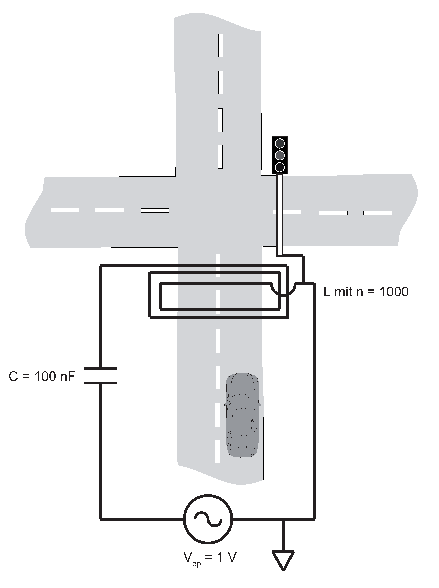
\includegraphics[width=\textwidth]{Abbildung19.png}
                \caption{Aufbau einer Induktionsschleife an einer Kreuzung.}
                \label{fig:abb19}
            \end{figure}
        \end{center}

        \subsection{Resonanzfrequenz}
        \paragraph{Aufgabe}
        Stellen Sie die Frequenz des Signalgenerators auf die eben ermittelte Resonanzfrequenz
        des LC-Schwingkreises ein und beobachten Sie die Spannung $U_2$ mit Hilfe des
        Oszilloskops. Setzen Sie Marker, um charakteristische Werte zu messen und nehmen
        Sie einen Screenshot auf.

        \paragraph{Protokoll}
        \begin{center}
            \begin{figure}[H]
                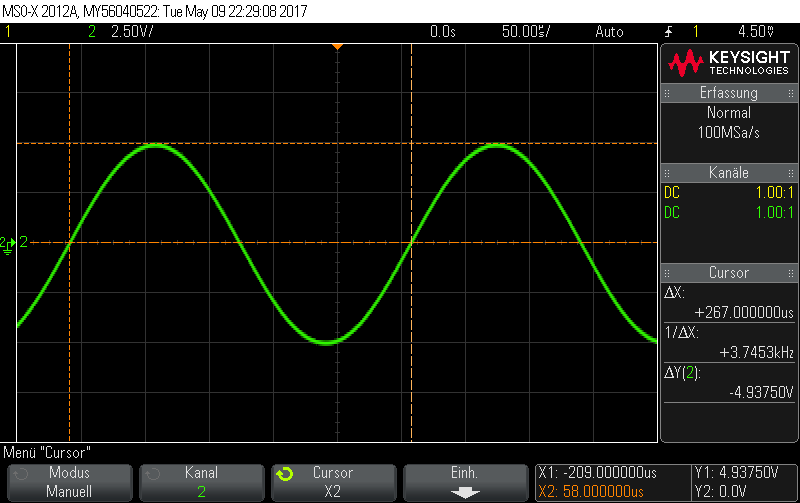
\includegraphics[width=\textwidth]{scope_24.png}
                \caption{Marker}
            \end{figure}
        \end{center}

        Das aufgezeichnete Signal hat eine Amplitude von $\hat{U} \approx 5
        \si{\volt}$ und eine Frequenz von $f \approx 3.7 \si{k\hertz}$.

        \subsection{Eisenkern}
        \paragraph{Aufgabe}
        Führen Sie nun einen Eisenkern in die Spule ein und beobachten Sie die Veränderung
        der Amplitude der Spannung $U_2$. Interpretieren Sie Ihre Beobachtung.

        \paragraph{Protokoll}
        \begin{center}
            \begin{figure}[H]
                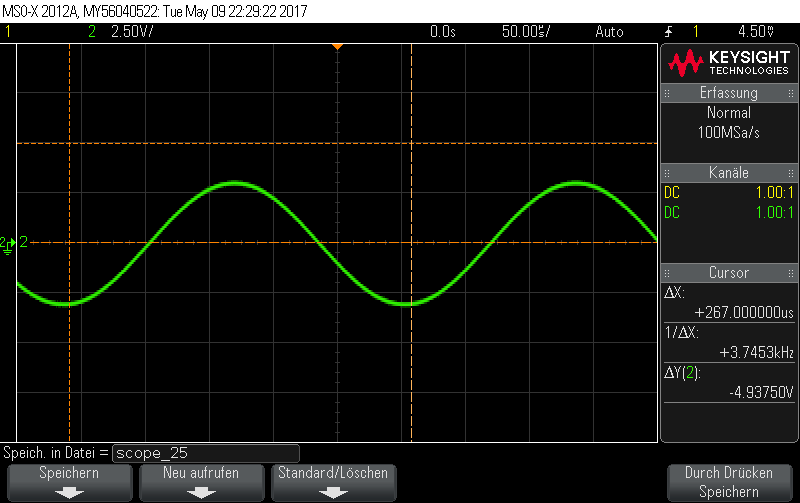
\includegraphics[width=\textwidth]{scope_25.png}
                \caption{Eisenkern halb in Spule}
                \label{fig:eisen1}
            \end{figure}
            \begin{figure}[H]
                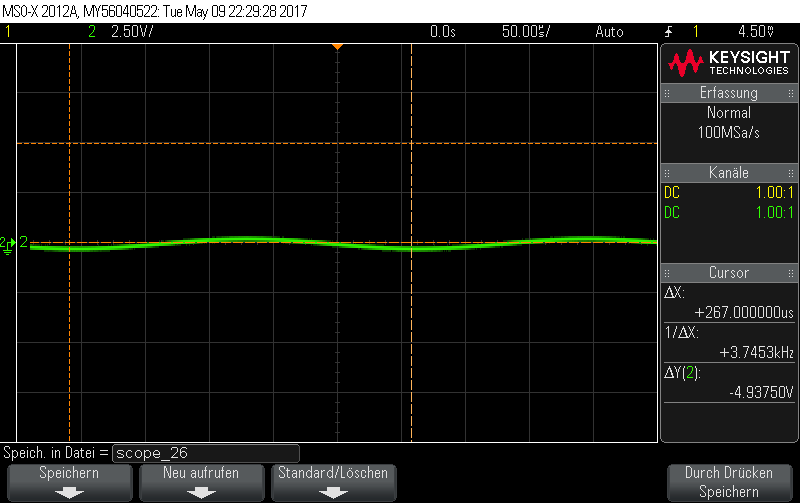
\includegraphics[width=\textwidth]{scope_26.png}
                \caption{Eisenkern vollständig in Spule}
                \label{fig:eisen2}
            \end{figure}
        \end{center}

        Wie in den Bildern~\ref{fig:eisen1} und~\ref{fig:eisen2} zu erkennen,
        verringert der Eisenkern die Amplitude des Signals.

        Dies lässt sich
        folgendermaßen Erklären:

        Es gilt:
        \begin{equation}
            f_0 = \frac{1}{2 \pi \sqrt{L C}}
        \end{equation}

        Da der Eisenkern die Induktivität der Spule erhöht, wird der Ausdruck im
        Zähler größer und die Resonanzfrequenz $f_0$ kleiner. Die zuvor am
        Funktionsgenerator eingestellte Frequenz von $3751 \si{\hertz}$ stimmt
        nun nicht mehr mit $f_0$ überein, was eine Verringerung der Amplitude
        zur Folge hat.

        \subsection{Frequenzsweep}
        \paragraph{Aufgabe}
        Wiederholen Sie nun den Frequenz-Sweep aus Versuch 3.3 mit Eisenkern in der
        Spule. Was stellen Sie fest? Interpretieren Sie Ihre Ergebnisse und erstellen Sie für
        Ihre Unterlagen eine Grafik des zweiten Frequenz Sweeps.

        \paragraph{Protokoll}

        \begin{center}
            \begin{figure}[H]
                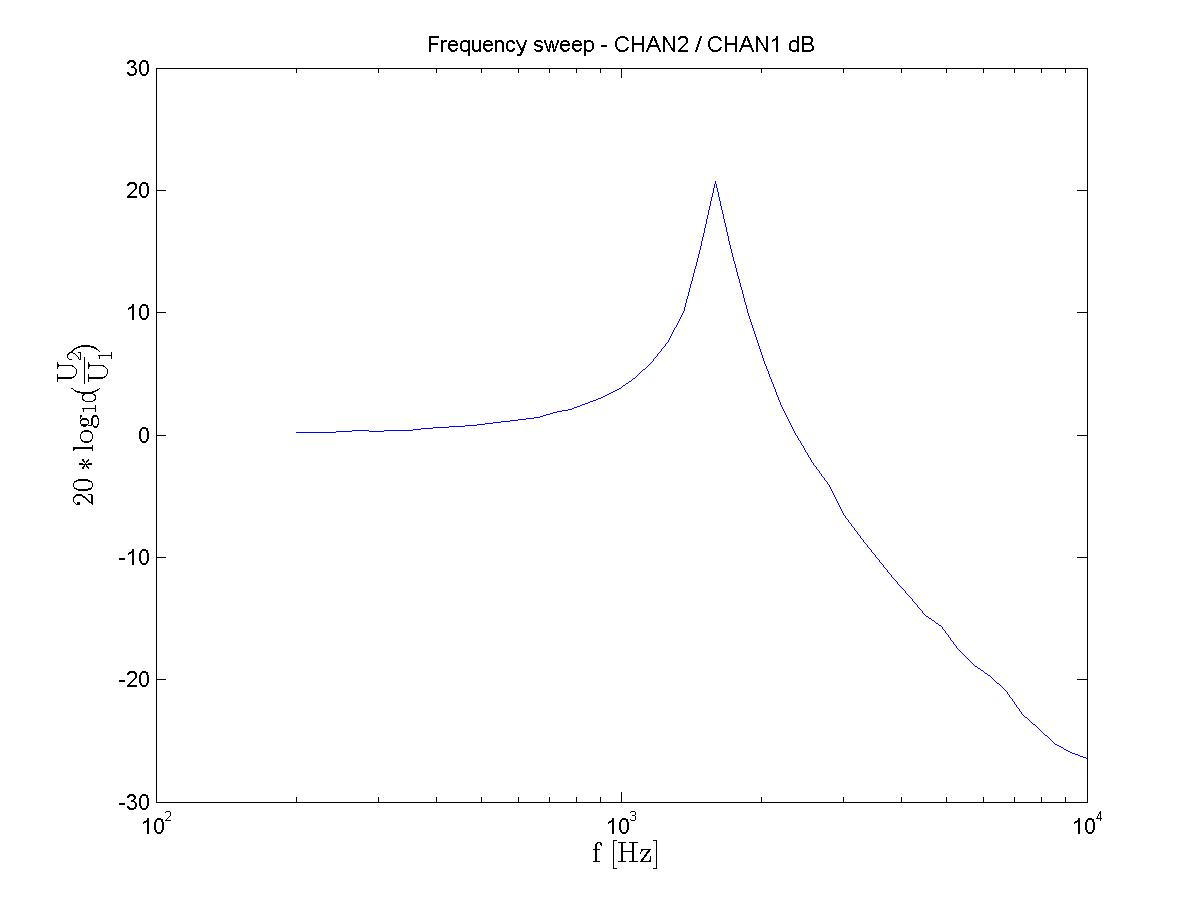
\includegraphics[width=\textwidth]{F_Sweep_2_frequencysweep_ylogxlog.jpg}
                \caption{Frequenzsweep}
                \label{fig:fsweep2}
            \end{figure}
        \end{center}
        Wie bereits in obiger Gleichung beschrieben, sorgt eine größere Induktivität
        für eine kleinere Resonanzfrequenz. Durch die größere Induktivität der
        Spule mit Eisenkern verschiebt sich also der Peak in Grafik~\ref{fig:fsweep2}
        nach links. Weiterhin ergibt sich aus dem Frequenz-Sweep:

        \begin{eqnarray}
            f_0 &\approx& 1100\si{\hertz}\\
            C &=& 100\si{n\farad}\\
            f_0 &=& \frac{1}{2 \pi \sqrt{L C}}\\
            \Leftrightarrow L &=& \frac{1}{{(f_0 2 \pi)}^2 C} \approx 0.21\si{\henry}
        \end{eqnarray}

        Die Induktivität wir also durch das Einführen des Eisenkerns ca.\ um einen Faktor
        $10$ größer.


        \section{Analyse einer unbekannten Schaltung}
        In diesem Versuch soll das Verhalten einer unbekannten Schaltung, einer sogenannten
        Blackbox (BB) untersucht werden. Hierzu steht Ihnen im Rahmen dieses Versuchs eine
        mit BB1 beschriftete Blackbox zur Verfügung. Alle möglichen Schaltungskombinationen,
        die sich im Inneren der Blackbox befinden können, sind in Abbildung~\ref{fig:abb21} dargestellt.
        Messen Sie die Transferfunktion der BB mit Hilfe des Schaltungsaufbaus in Abbildung
        \ref{fig:abb20}. Verwenden Sie hierzu einen Sweep mit einer unteren Frequenz von $1\si{\hertz}$, einer oberen
        Frequenz von $250\si{k\hertz}$ und einer Auflösung von $200$ Punkten.

        \begin{center}
            \begin{figure}[H]
                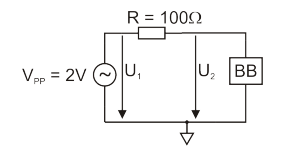
\includegraphics[width=\textwidth]{Abbildung20.png}
                \caption{Messaufbau zum Analysieren der BB}
                \label{fig:abb20}
            \end{figure}
            \begin{figure}[H]
                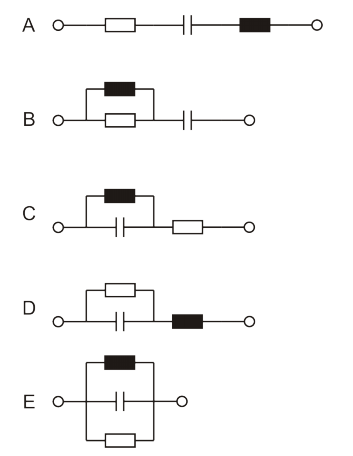
\includegraphics[width=\textwidth]{Abbildung21.png}
                \caption{Mögliche Schaltungen der BB}
                \label{fig:abb21}
            \end{figure}
        \end{center}

        \subsection{Schaltung bestimmen}
        \paragraph{Aufgabe}
        Bestimmen Sie welche Schaltung aus Abbildung 21 in der BlackBox enthalten ist.
        Gibt es mehrere Möglichkeiten? Hinweis: Verwenden Sie Ihre Abschätzungen aus
        der Versuchsvorbereitung (Abschnitt 2.4).

        \paragraph{Protokoll}
        \begin{center}
            \begin{figure}[H]
                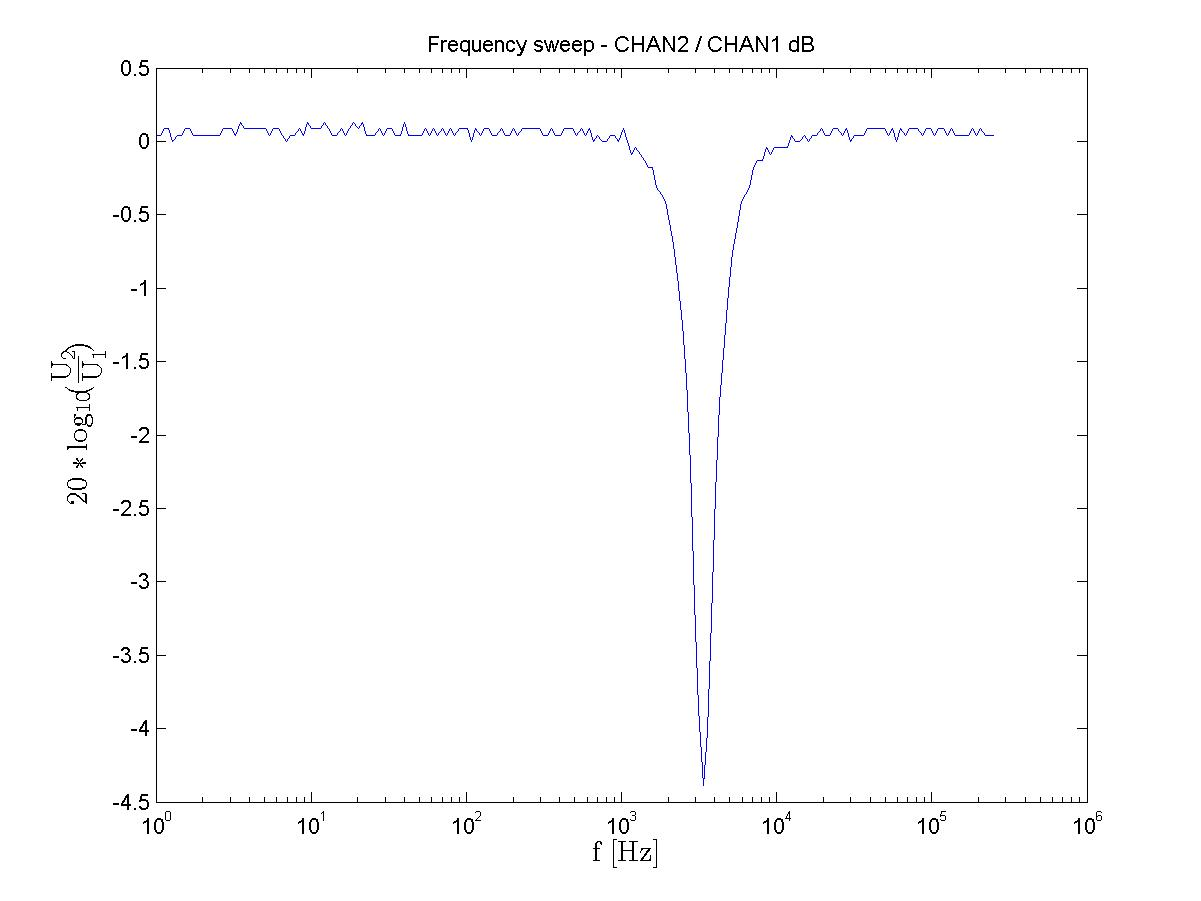
\includegraphics[width=\textwidth]{F_Sweep_BB_frequencysweep_ylogxlog.jpg}
                \caption{Frequenzsweep der BB}
            \end{figure}
        \end{center}

        Für $f \rightarrow 0$ bzw. $f \rightarrow \infty$ beträgt der logarithmische
        Wert der Übertragungsfunktion 0dB. Das heißt: $U_1 \approx U_2$.
        Daraus folgt, dass über der BB viel Spannung abfallen muss, was bedeutet,
        dass sie eine hohe Impedanz besitzt.

        Für den Resonazfall zeigt das Bode-Diagramm einen deutlichen Einbruch,
        was bedeutet, dass $U_2 < U_1$ sein muss. Diese wiederum bedeutet, das die
        BB bei der Resonanzfrequenz eine vergleichsweise geringe Impedanz haben muss.

        Schaltung A weist genau dieses Verhalten auf, weswegen die BB aus einer
        Reihenschaltung von Widerstand, Kondensator und Spule bestehen muss.

        \subsection{Wieso keine andere Schaltung?}
        \paragraph{Aufgabe}
        Begründen Sie für jede andere Schaltung, wieso diese nicht in der BB enthalten
        sein kann. Verwenden Sie für Ihre Begründung das Übertragungsverhalten bei einer
        sehr kleinen Frequenz, bei der Resonanzfrequenz und bei der oberen Frequenz des
        Messbereiches.

        \paragraph{Protokoll}
        \textbf{Schaltung B:} Verhält sich nicht symmetrisch. Für $f \rightarrow 0$
        und $f \rightarrow \infty$ verhält sich die Schaltung nicht gleich.

        \textbf{Schaltung C:} Bei der Resonanzfrequenz müsste sich das Bode-Diagramm
        der 0 annähern, was im dargestellten Diagramm nicht der Fall ist.

        \textbf{Schaltung D:} Verhält sich nicht symmetrisch. Für $f \rightarrow 0$
        und $f \rightarrow \infty$ verhält sich die Schaltung nicht gleich.

        \textbf{Schaltung E:} Bei den Grenzfällen $f \rightarrow 0$ und
        $f \rightarrow \infty$ müsste sich das Diagramm der $-\infty$ annähern,
        was im dargestellten Diagramm nicht der Fall ist.
\end{document}
